


%-------------------------

\newpage

%\section[From Paris to Zhuhai][De Paris à Zhuhai]{From Paris to Zhuhai}{De Paris à Zhuhai}
\section{From Paris to Zhuhai}{De Paris à Zhuhai}

\label{sec:casestudies}

%-------------------------


Nous développons dans cette section des cas d'étude géographique à l'échelle métropolitaine, que nous choisissons très différents pour montrer la diversité des situations possibles mais aussi les motifs récurrents généraux qui pourraient se dégager. Il s'agit de la métropole du Grand Paris, et de la mega-région urbaine du Delta de la Rivière des Perles dans le sud de la Chine.


%-------------------------

%%%%%%%%%%%%%%%%%%%%%%%%
%\subsection[Greater Paris][Grand Paris]{Greater Paris: History and current Issues}{Le Grand Paris : histoire et enjeux}
\subsection{Greater Paris: History and current Issues}{Le Grand Paris : histoire et enjeux}


La région parisienne est une bonne illustration de la complexité des interactions entre réseaux de transports et territoires, au cours du temps et à l'échelle intermédiaire d'une région métropolitaine globalement monocentrique. \cite{gilli2005bassin} rappelle l'importance de l'hinterland du Bassin Parisien et l'importance de ne pas considérer l'hypercentre de manière isolée. Si la moyenne couronne possède un certain niveau de polycentricité, notamment grâce à l'effet des villes nouvelles qui sont d'importants pôles d'emplois locaux~\cite{berroir2005contribution} qui même s'il a rapidement divergé des intentions planificatrices~\cite{es119}, est bien réel, le Bassin Parisien étendu peut être également lu ayant un certains nombre de centres importants à une heure de Paris : Chartres, Orléans, Rouen, Reims et Lille grâce à la grande vitesse. Le rôle des différentes infrastructures de transport dans les différentes dynamiques économiques en Ile-de-France n'est pas trivial, comme le montre~\cite{PADEIRO201344} qui cherche à expliquer statistiquement la croissance de l'emploi entre 1993 et 2008 dans les moyennes et petites communes franciliennes en fonction de la proximité à une infrastructure : les effets dépendent à la fois du mode (autoroute ou aéroport) mais aussi du secteur économique considéré. Réciproquement, les développements successifs, généralement par ruptures, que nous détaillerons par la suite, sont liés à des dynamiques de planification et des processus de gouvernance qu'il convient de comprendre de manière intégrée. La métropole parisienne, qu'on désignera par \emph{Grand Paris}, et sa région d'influence élargie, témoignent ainsi de relations complexes entre territoires et réseaux.




\paragraph{Governance}{Gouvernance}

\cite{gilli2009paris} propose en 2009 un diagnostic de la situation institutionnelle de la région parisienne, et des pistes pour une approche couplée entre gouvernance et aménagement. La préfiguration de ``l'instauration d'un acteur collectif métropolitain'' correspond à la métropole du Grand Paris qui sera inaugurée 7 ans plus tard, puisque le conseil métropolitain est mis en place fin 2016. Son effectivité concrète reste quasi-nulle au moment de l'écriture, confirmant une certaines inertie des structures de gouvernance, qui a nécessairement un impact sur celle des réseaux de transport. La mise en place de ce nouveau niveau de gouvernance a été disséquée plus récemment toujours par \noun{Gilli} dans~\cite{gilli2014gouverner}, où il la situe dans un contexte plus large socio-économique et urbain, en quelque sorte un diagnostic territorial qui explique certains aspects de ce besoin de mutation. En perte de vitesse sur le plan de l'aménagement, mais aussi sur le plan social au vu d'inégalités socio-économiques locales très fortes, la métropole a besoin de se réinventer, et se nouveau souffle se cristallise naturellement dans le Grand Paris, c'est à dire ``l'avenir de Paris est sa banlieue''. Cette initiative se concrétise par la convergence d'une auto-organisation des élus locaux, et d'une redéfinition du rôle de l'état, voulue centralisatrice jusqu'en 2012 puis laissant la place libre à la gouvernance métropolitaine avec le nouveau gouvernement, même si les projets lancés et les financements restent les mêmes dans les grandes lignes : le projet du Grand Paris Express est un compromis entre la solution voulue par l'état et celle poussée par la région. Suivant~\cite{desjardins2016grand}, si la structure de gouvernance métropolitaine est aujourd'hui toujours relativement impuissante, et si l'oubli de l'aspect social du développement métropolitain est toujours très présent, ces mutations témoignent toutefois d'un changement structurel profond dans l'organisation de la région.




\paragraph{Grand Paris Transportation Network}{Réseau de Transport du Grand Paris}

L'histoire du développement du réseau de transport de la métropole francilienne est rappelée dans~\cite{beauguitte:halshs-01068589}. La particularité centralisatrice française a conduit à une structure particulière du réseau ferré à l'échelle nationale, mais aussi à celle régionale. La domination de Paris a en effet fortement marqué la structuration du réseau de transport au cours des différentes périodes historiques où il a subit des évolutions conséquentes. Avant 1975, la distribution de l'accessibilité est clairement centralisée et le centre de Paris fortement congestionné. La mise en place du réseau RER entre 1975 et 1990, même si elle ne suit pas la volonté initiale de Delouvrier qui comprenait un plus grand nombre de branches transversale, permet la concrétisation d'un certain niveau de polycentrisme grâce à la construction conjointe des Villes Nouvelles. La période qui suivra jusqu'à aujourd'hui visera surtout à des désenclavements, mais aucun changement majeur d'accessibilité n'est observé. Les schémas directeurs successifs, qui aboutiront au SDRIF de 2013~\cite{sdrif2013}, préfigurent le futur réseau du Grand Paris Express, qui aura un impact crucial en terme de cohésion territoriale en favorisant les liaisons de banlieue à banlieue qui sont les plus problématique dans le réseau actuel. De plus, le schéma se veut pensé de manière intégrée, par densification autour des gares et articulation des opérations d'aménagement et les nouvelles infrastructures.




\paragraph{Impact of the Grand Paris Express}{Impact du Grand Paris Express}


Les impacts immédiats d'une nouvelle de transport en terme d'accessibilité concernent généralement des territoires bien plus larges que les zones où la ligne et ses stations sont implantées : les motifs d'accessibilité sont dus aux propriétés topologiques du réseau et celles-ci sont fortement discontinues en fonction de la structure du graphe. Illustrons le cas des lignes du Grand Paris Express et de leur impact direct sur l'accessibilité régionale. La Fig.~\ref{fig:casestudies:gpe} cartographie les gains de temps moyens permis par ce projet sur les départements métropolitains (75, 92, 93 et 94)\footnote{voir la section~\ref{sec:grandparisrealestate} pour le détail de la méthodologie de calcul.}, avec le tracé le plus récent pour l'ensemble des lignes. On observe, conformément à l'analyse de~\cite{beaucire2013grand}, un rééquilibrage des différentiels d'accessibilité entre Est et Ouest. A distance égale du centre, l'accessibilité temporelle moyenne est plus élevée pour la Seine-Saint-Denis et le Val-de-Marne que pour les Hauts-de-Seine. La carte des gains temporels moyens montre les gains plus grands également pour ces deux départements. Des communes socio-économiquement défavorisées comme Aulnay sont bénéficiaires des plus grands gains de temps. La ligne 16 est en effet précisément dédiée au désenclavement du nord-est de la Seine-Saint-Denis~\cite{desjardins2016grand}. La création de liaisons de banlieue à banlieue est un aspect majeur de ce désenclavement et est voulue comme un moteur de l'émergence de nouvelles centralités, vers une métropole toujours plus polycentrique, dans la lignée de la politique d'aménagement des villes nouvelles, pour ne plus parler de proche banlieue mais de quartiers faisant partie intégrante du Grand Paris. Les effets peuvent cependant être mitigés selon les zones : \cite{l2013grand} montre que le Grand Paris Express induira un accès direct à un plus grand nombre d'emplois pour un nombre significatif de chômeurs en petite couronne, mais que les écarts avec la grande couronne seront accentués et qu'il existe des risques de décrochage de certaines communes lointaines mal desservies. L'un des enjeux cruciaux pour la construction du Grand Paris est de veiller à ne pas obtenir une métropole à plusieurs vitesses, et de tirer parti de la connectivité accrue à plusieurs échelles (internationale, nationale, régionale, métropolitaine) pour réduire les inégalités territoriales plutôt que les accroitre. Le nouveau réseau semble contribuer à cette dynamique, sous condition d'un développement territorial coordonné, permettant la concrétisation des gains immédiats d'accessibilité en terme de transformation territoriale. Il n'existe pas de méthode pouvant prévoir celle-ci de manière sûre comme mous l'avons déjà développé. L'un des enjeux de notre travail par la suite sera de clarifier empiriquement des situations dans lesquelles des dynamiques fortement couplées relevant de cette problématique pourront être mises en évidence puis à travers des modèles d'isoler des processus et des conditions permettant telle ou telle situation.



%%%%%%%%%%%%%%%%%%%
\begin{figure}
	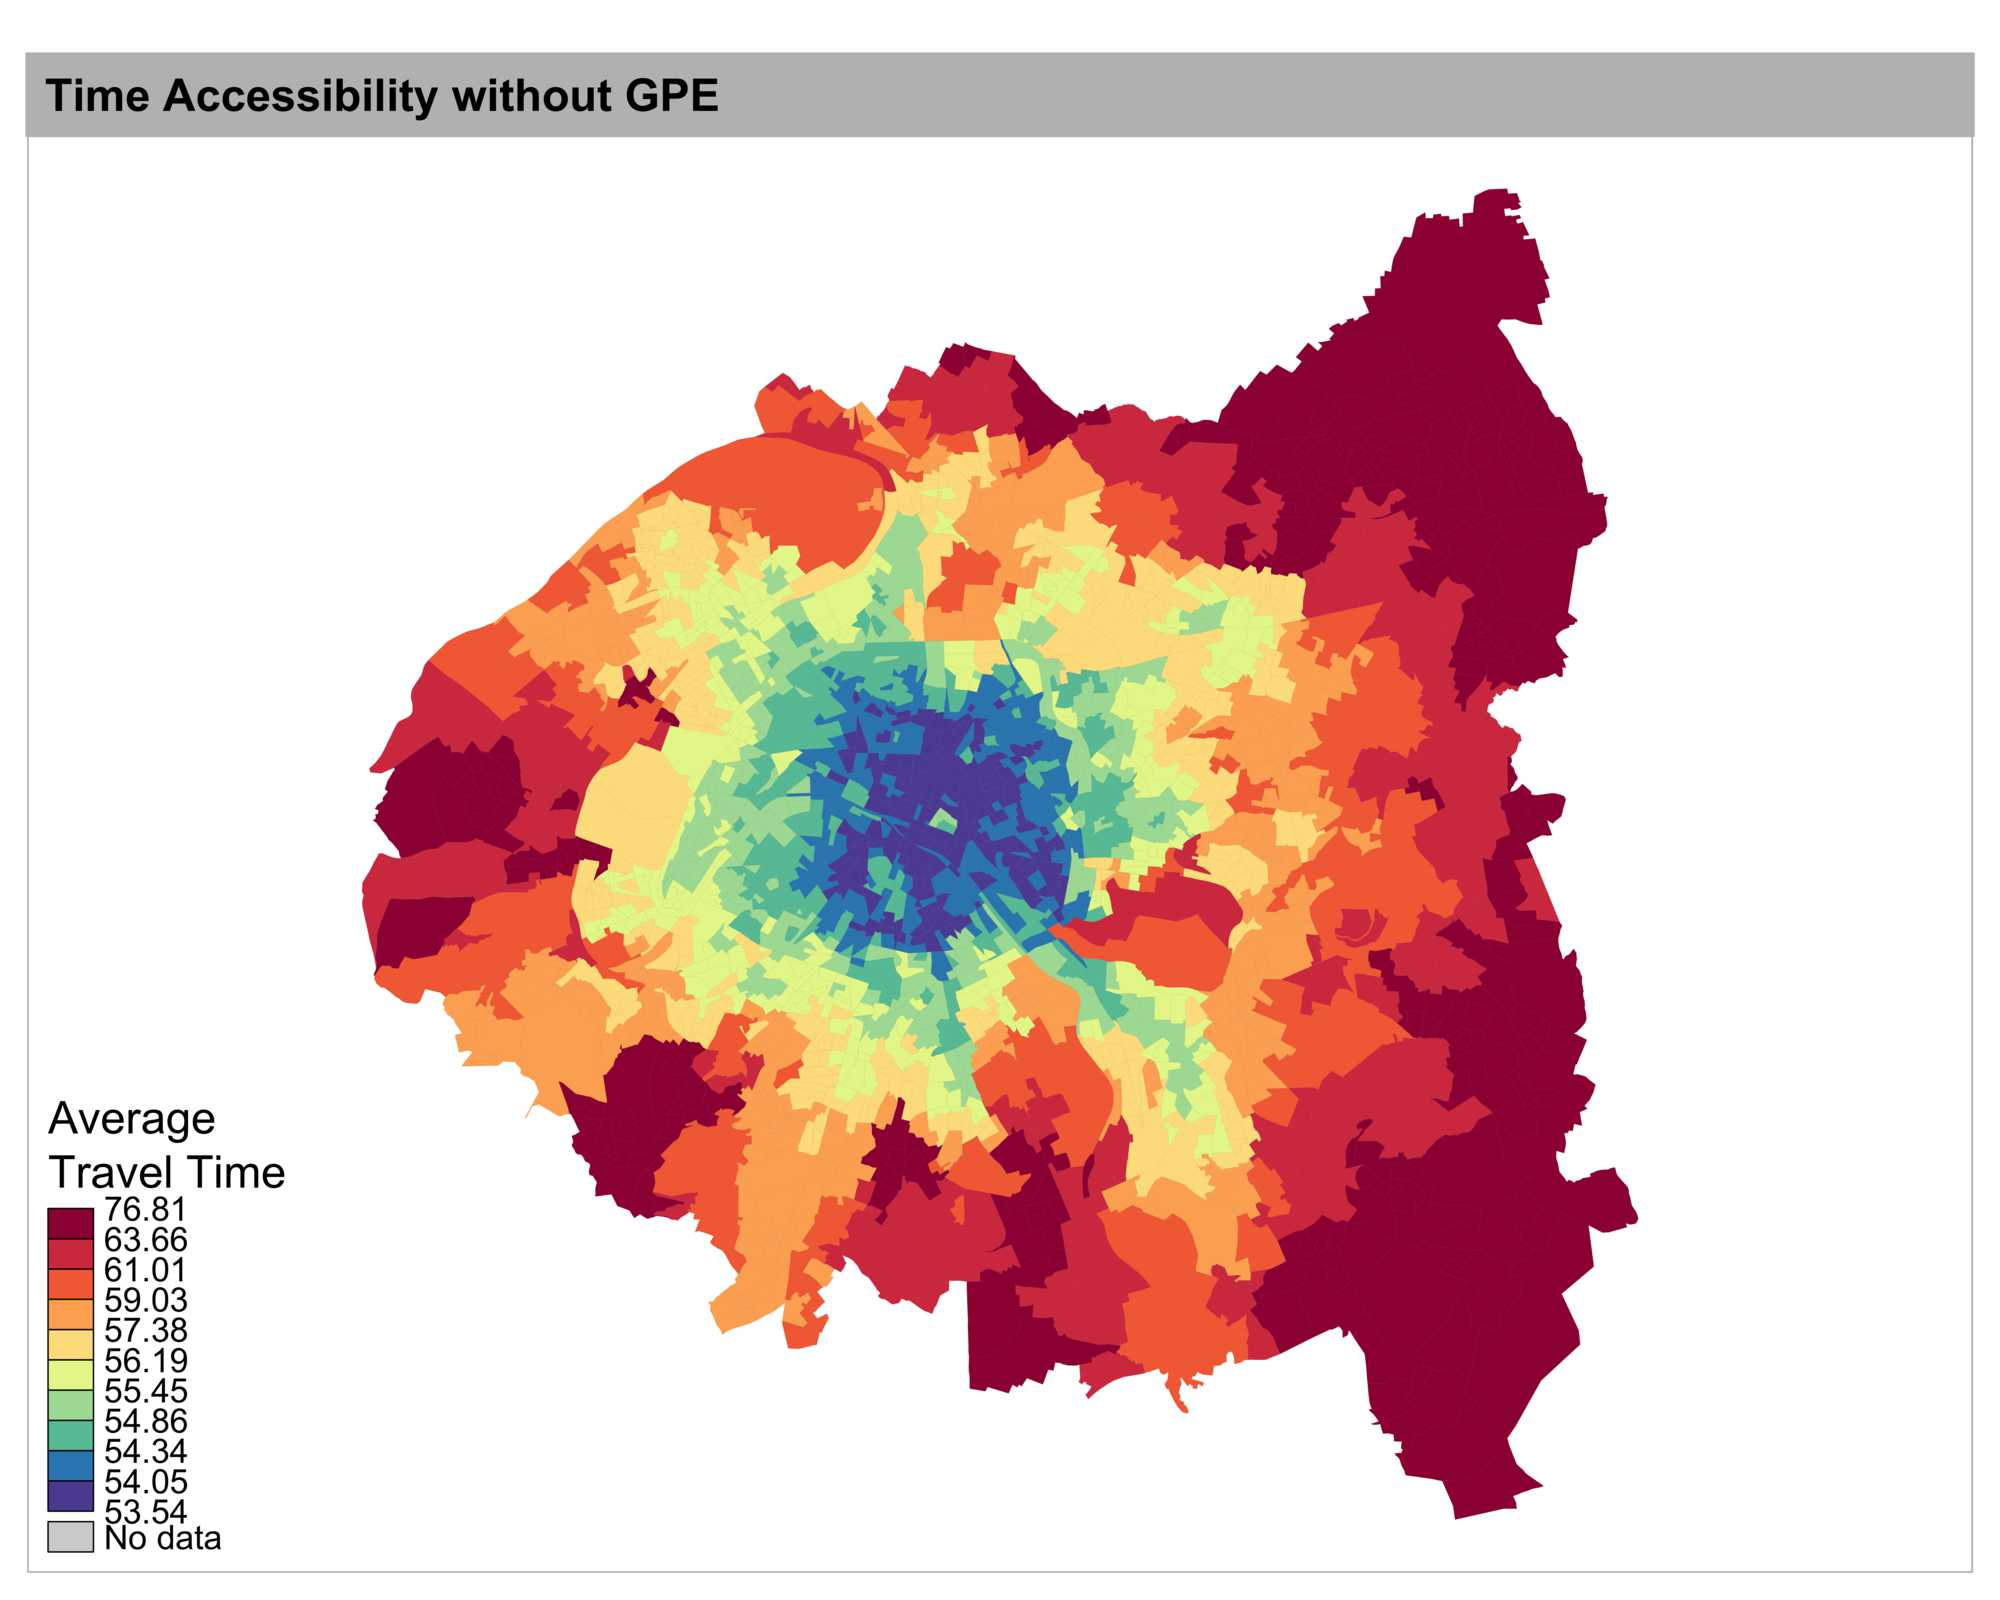
\includegraphics[width=0.8\linewidth]{Figures/CaseStudies/timeaccess_metropole}\\
	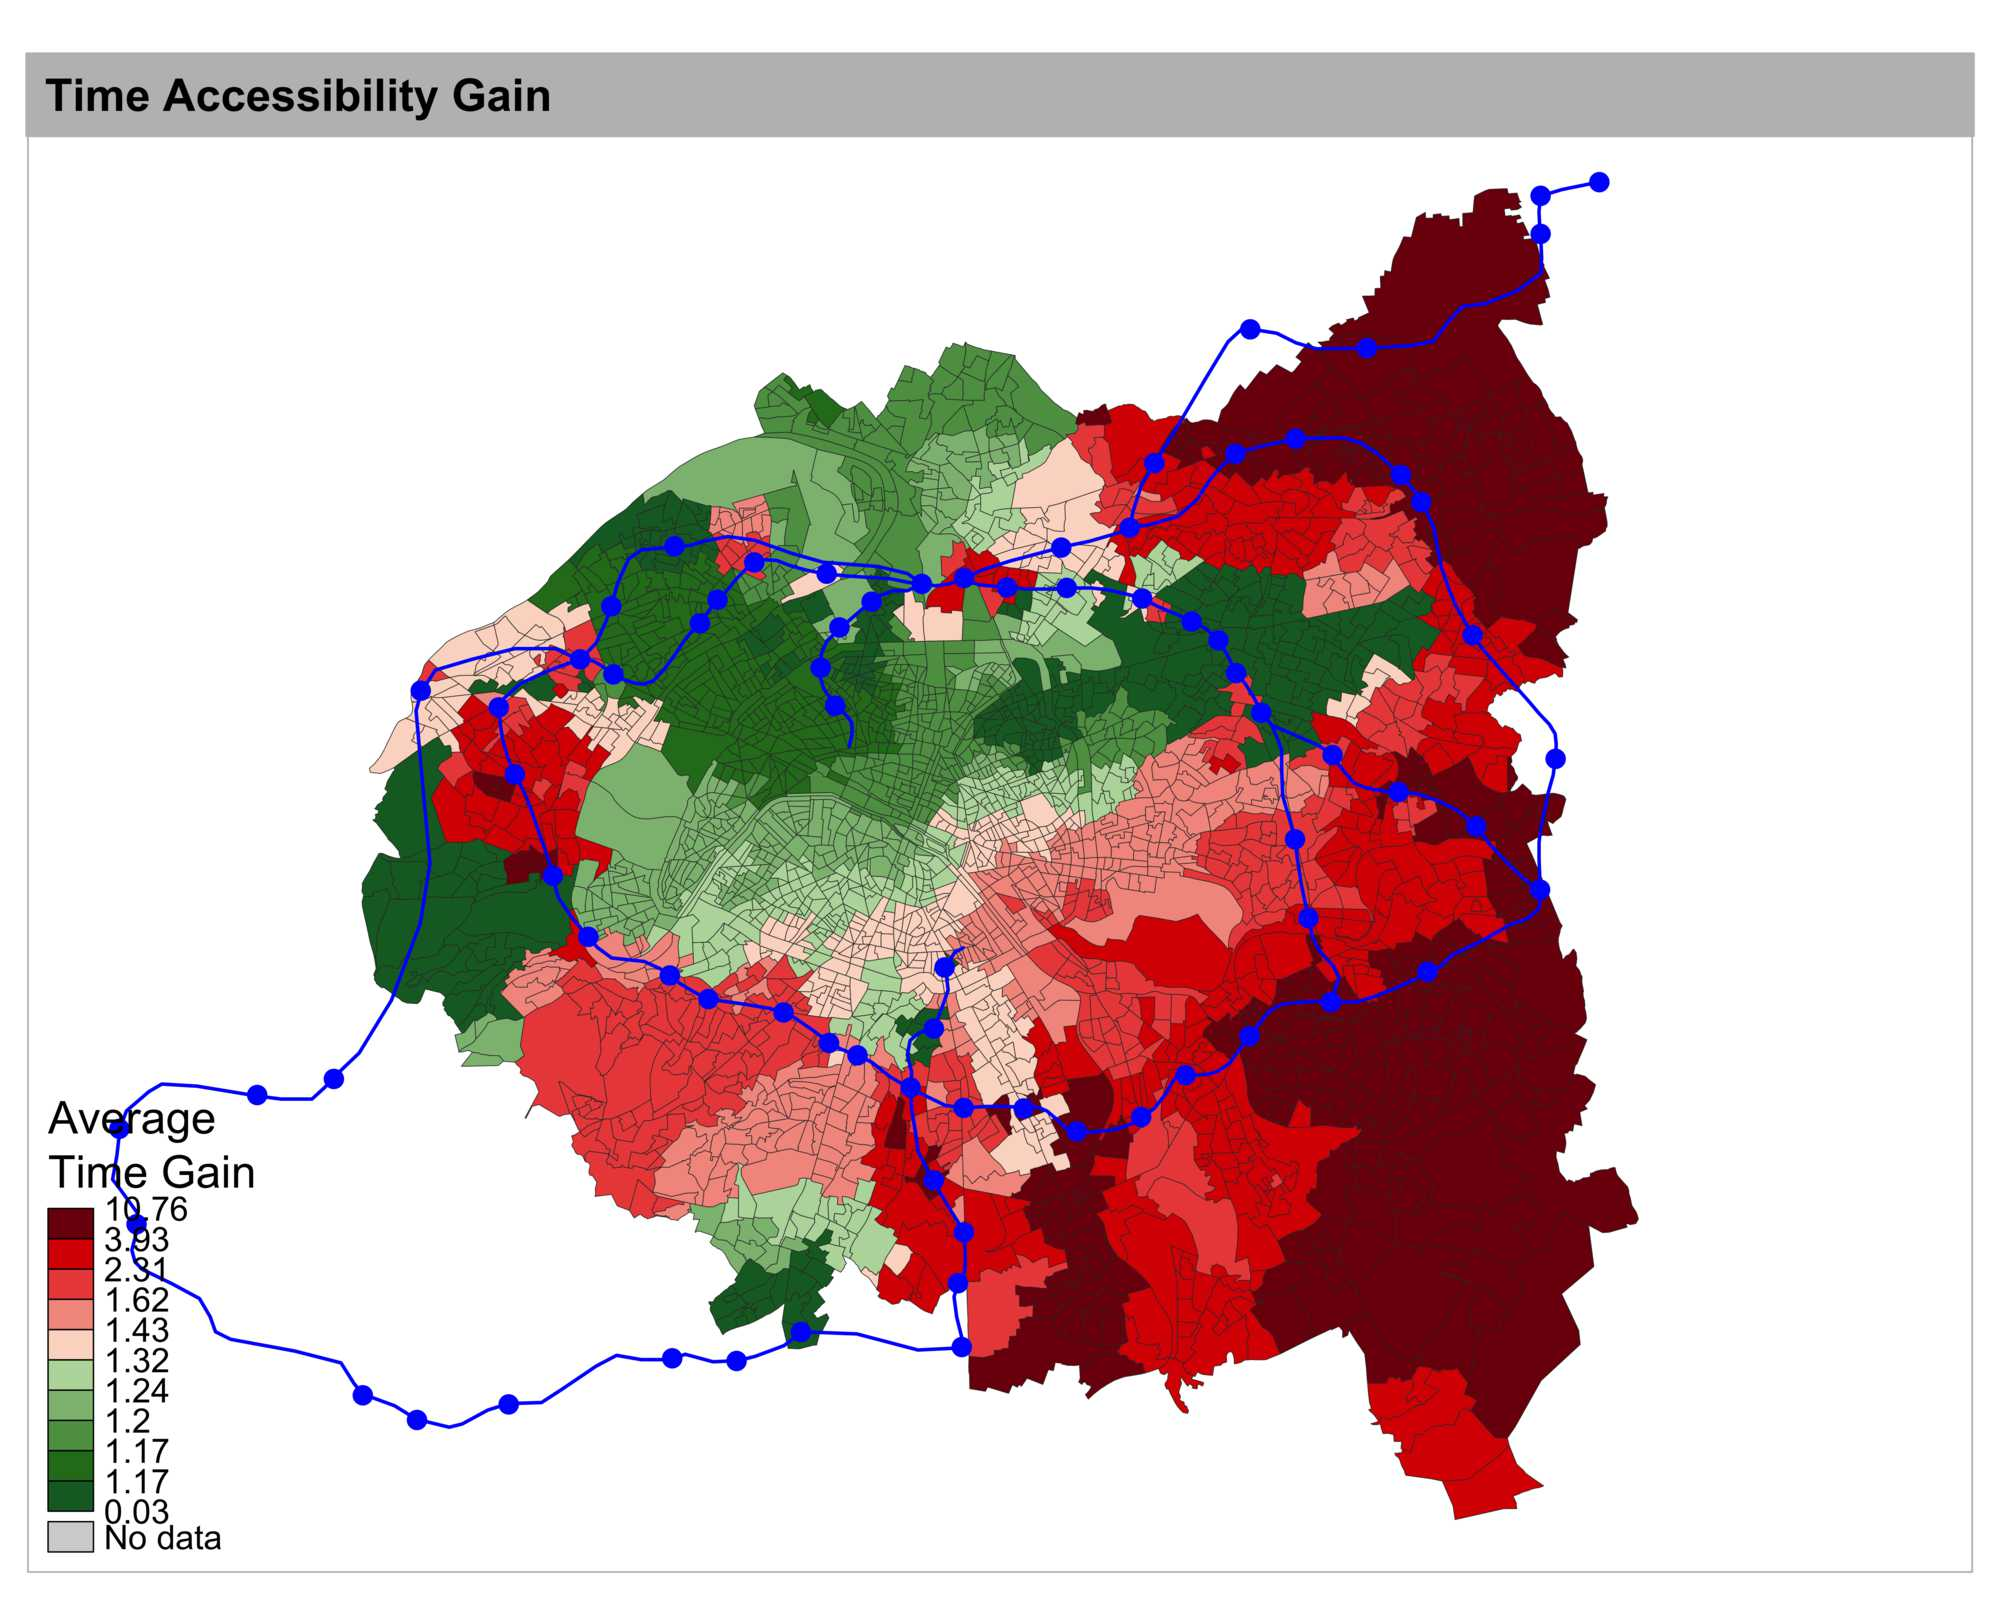
\includegraphics[width=0.8\linewidth]{Figures/CaseStudies/timegain_metropole}
	\caption[Impact of \emph{Grand Paris Express}][Impact du Grand Paris Express]{\label{fig:casestudies:gpe}}{\textbf{Impact des lignes du GPE sur l'accessibilité temporelle.} \textit{(Haut)} Temps moyen de trajet vers l'ensemble des communes d'Ile-de-France, par transports en commun uniquement, pour les départements métropolitains ; \textit{(Bas)} Gains de temps permis par l'ensemble des lignes du GPE, avec le trajet des lignes.\label{fig:casestudies:gpe}}
\end{figure}
%%%%%%%%%%%%%%%%%%%




%-------------------------


%%%%%%%%%%%%%%%%%%%%%%%%
%\subsection[Pearl River Delta][Le Delta de la Rivière des Perles]{Pearl River Delta: new urban regimes and mega-city regions}{Le Delta de la Rivière des Perles : nouveaux régimes urbains et Mega-région urbaine}
\subsection{Pearl River Delta}{Le Delta de la Rivière des Perles}


\paragraph{New urban regimes and mega-city regions}{Nouveaux régimes urbains et Mega-région urbaine}

\bpar{}{
Si la notion de megalopolis peut être tracée jusqu'à \noun{Gottmann}~\cite{gottmann1964megalopolis}, et qu'elle est à l'origine de celle de \emph{Mega-city Region} (MCR) consacrée par \noun{Hall}~\cite{hall2006polycentric}, il est clair que cette dernière est toujours plus d'actualité avec l'apparition récente de nouveaux régimes, notamment par l'urbanisation accélérée dans des pays à forte croissance économique et en mutation très rapide comme la Chine~\cite{swerts2015megacities}. Le second cas que nous développons ici rentre dans cette catégorie : le Delta de la Rivière des Perles est une des illustrations classiques de la structure d'une MCR fortement polycentrique. Historiquement initialement composé de Guangzhou uniquement, le développement de Hong-Kong puis la mise en place Zones Economiques Spéciales (\cn{经济特区}) dans le cadre des politiques d'ouverture de \noun{Deng Xioaping}, a conduit à un développement extrêmement rapide de Shenzhen, et dans une moindre mesure de Zhuhai. La province du Guangdong dans lequel le PRD se situe intégralement a actuellement le plus fort PIB régional de Chine, et la MCR regroupe une population d'environ 60 millions (les estimations fluctuant fortement selon la définition prise de la MCR et la prise en compte de la population flottante). Le phénomène de migration des campagnes est très présent dans la région et une ville comme Dongguan a par exemple basé son économie sur des manufactures employant ces travailleurs migrants.
}


\bpar{}{
\cite{Ye2014200} analyse les actions de gouvernance métropolitaine à l'échelle de centres de la MCR, et plus particulièrement comment les communes de Guangzhou et Foshan ont progressivement accru leur coopération pour former une zone métropolitaine intégrée, pouvant ainsi fortement influencer le développement des transports par exemple et permettant la mise en place d'un réseau connecté. Une forte tension entre des processus émergents par le bas, et un dirigisme d'état relativement fort en Chine, se répercutant de l'Etat central, au gouvernement provincial jusqu'aux gouvernements locaux, a permis la mise en place d'une telle structure. La compétition avec les autre villes de la MCR reste très forte, et la logique d'intégration de la MCR est partiellement guidée par la région seulement. La nature particulière des ZES de Shenzhen et Zhuhai, liée aux relations privilégiées avec les Zones Administratives Spéciales de Hong-Kong et Macao, qui n'ont été réintégrées à la République Populaire qu'à la fin du millénaire et conservent un certain niveau d'indépendance en termes de gouvernance, complique encore les jeux d'acteurs au sein de la région. La question d'un niveau de gouvernance qui expliquerait tel ou tel processus urbain est épineuse : \cite{liao2017ouverture} interprète les transferts progressifs des initiatives économiques du pouvoir central vers les autorités locales comme une forme de gouvernance multi-niveau. Dans le cadre des transports pour la MCR, il n'existe pas d'autorité d'organisation des transports, et chaque commune gère indépendamment le réseau local, tandis que les connections entre villes sont assurées par le réseau de train national. Cela conduit à des situations particulières dans lesquelles des zones se retrouveront très enclavées, avec une hétérogénéité très forte localement. Ainsi, la pointe sud de la ville de Guangzhou qui sert d'accès direct à la mer, est plus proche géographiquement du centre de Zhongshan, mais un lien direct par transports en commun est difficile à envisager, alors que la zone est bien reliée au centre de Guangzhou par la ligne de métro. Une situation similaire s'observe au terminus de la ligne 11 de Shenzhen, pour le quartier limitrophe de Dongguan, ce dernier étant très peu accessible. Cette situation serait cependant transitoire, étant donné les infrastructures déjà en construction et celles planifiées sur un plus long terme : le métro de Shenzhen, qui couvre aujourd'hui 285km, est planifié jusqu'à 30 lignes et 1142km en 2030~\cite{shenzhen2016plan}. Il est clair que ces développements suivent pour la majorité un développement urbain existant, une question cruciale est la volonté et la capacité à contenir l'étalement urbain et structurer les futurs développements autour de ce nouveau réseau, dans l'esprit d'une intégration volontaire entre urbanisme et transport de type Transit Oriented Development. Différents terminus seront connectés au metro de Dongguan, et de nouvelles lignes intercités structureront les déplacements de plus longue portée, ce qui fera du Delta dans un horizon temporel proche une MCR relativement bien intégrée en termes de transports en communs.
}


\paragraph{Impact of the Zhuhai-Hong-Kong-Macao bridge}{Impact du Pont Zhuhai-Hong-Kong-Macao}

Un projet iconique d'infrastructure de transport dans la région est le pont fermant l'embouchure du Delta, reliant Zhuhai et Macao à Hong-Kong. En réalité un Pont-tunnel. La longueur de la traversée est de 36.5km, ce qui en fait un ouvrage d'art exceptionnel. L'ouverture au traffic a été retardée de plusieurs années et est prévue finalement pour fin 2017\footnote{voir \texttt{http://www.hzmb.org/cn/default.asp}}. \cite{zhou2016medium} montre que les changements de motifs d'accessibilité attendus pour l'Ouest du Delta sont relativement forts, et ceux-ci peuvent potentiellement induire de fortes bifurcations dans les trajectoires des villes. La nécessité du projet est supportée par une narration de fort bénéfice économique dans le cadre des politiques d'ouverture, ainsi que par un bénéfice social pour l'Ouest notamment. Par exemple, Zhuhai se positionne comme un nouveau pivot entre Hong-Kong et l'ouest. L'équilibrage d'accessibilité s'opère cependant pour le mode routier uniquement, ce qui conduit à questionner ses impacts potentiels : d'une part l'accès systématique à l'automobile reste réservé à une partie de la population seulement, d'autre part les externalités négatives de congestion peuvent rapidement modérer les gains d'accessibilité. Les impacts à moyen et long terme du pont sont ainsi difficile à estimer, une piste étant de poser le problème différemment et de chercher comprendre la dynamique du système métropolitain de manière intégrée, comme nous l'évoquerons en~\ref{sec:lutetia}.





%-------------------------


%%%%%%%%%%%%%%%%%%%%%%%%
\subsection{Comparability of case studies}{Comparabilité des études de cas}


La possibilité de transfert des modèles urbains est délicate, et la particularité Est-asiatique a déjà été montrée pour la structure économique, et comment celle-ci ne peut être interprétée de manière simple par une séparation des processus microscopiques et macroscopiques comme certaines lectures rapides et idéologiquement orientée ont pu le faire, comme la vision de la Banque Mondiale~\cite{amsden1994isn}. La comparabilité de systèmes urbains est une question ouverte au centre des enjeux de la Théorie Evolutive Urbaine, et est par exemple liée au caractère ergodique de ces systèmes : si la trajectoire d'une ville dans le temps capture l'ensemble des états urbains possibles, alors les différentes villes sont différentes manifestations du même processus stochastique à différentes périodes, et un ensemble de villes permettrait d'avoir une idée des trajectoires temporelles. Intuitivement ce n'est pas le cas, et la Théorie Evolutive postule en effet la non-ergodicité~\cite{pumain2012urban}, que nous étudierons plus en détail en~\ref{sec:staticcorrelations}.







\stars




